\chapter{Modèles à circuits électriques pour les cellules PV}

\section{Introduction}
Dans ce chapitre, nous parlerons des circuit électriques à éléments localisés qui sont utilisés pour la modélisation des cellules PV. Plus précisément, on discutera les modèles simple et double diode, les rôles et l'influence de chaque paramètre sur le modèle et finalement les techniques utilisées dans la littérature pour l'identification et l'estimation de ces paramètres.

\section{Généralités}

Fondamentalement, les cellules PV se composent de deux couches de semi-conducteurs à dopages différents, la jonction de ces deux couches étant exposée à la lumière incidente. En effet, les électrons dans la bande de conduction sont capables d'être transférés vers la bande de valence tant que l'énergie du photon incident $E = h \nu$ est supérieure à la largeur de la bande interdite $E_g = E_c - E_v$. Toute l'architecture d'une cellule quelconque vise à profiter le plus que possible de la différence de tension engendrée par les excitons séparés par le champ électrique dans la zone de déplétion (ou zone de charge d'espace) (figure \ref{fig:pn}). Par exemple, les contacts supérieurs sont des oxydes transparents conductifs (dit couche fenêtre) pour laisser passer le plus grand nombre de photons possible vers la couche absorbante de la cellule. Pour quelques cellule en couche mince, le contact arrière se compose d'une couche réfléchissante (ZnO et Ag ou Al) qui renvoie la lumière vers la couche absorbante pour minimiser davantage les pertes en lumière transmise \cite{Chopra2004}.

\begin{figure}
  \begin{center}
    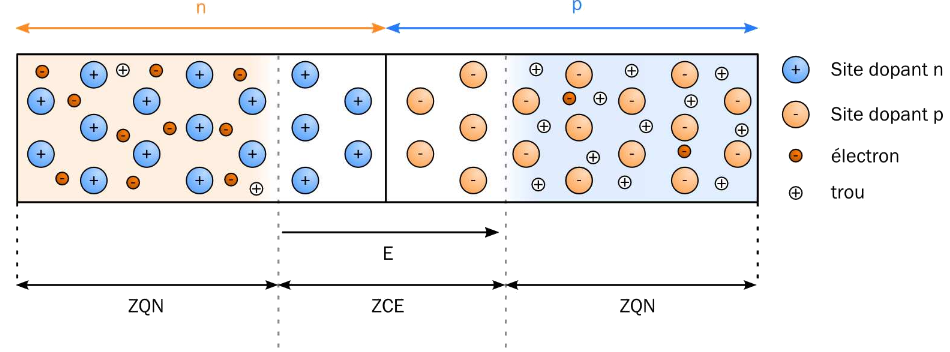
\includegraphics[width=.7\textwidth]{resources/pn.PNG}
    \caption{Schéma d'une jonction PN représentant : la zone de charge d'espace
(ZCE), les zones quasi-neutres (ZQN), les différents porteurs de charge, les sites dopants et le champ électrique E - Roger, 2013 \cite{Roger2013}.}
    \label{fig:pn}
  \end{center}
\end{figure}  

En fait, le comportement électrique d'un telle cellule en l'absence de la lumière est identique à celui d'une diode PN classique dont la caractéristique est décrite par l'équation de Shockley (équation \ref{eq:shockley}). Dans cette formule, le $I_0$ est le courant de saturation de la diode, $q$ la charge élémentaire $e^{-}$, $a$ le facteur d'idéalité, $k$ la constante de Boltzmann et $T$ la température de la cellule. Parfois on utilise la notion de \textit{voltage thermique}: $V_t = \frac{kT}{q}$.

\begin{equation}
\label{eq:shockley}
  I_D = I_0 \bigg[e^{\big(\frac{qV}{akT}\big)} - 1\bigg]
\end{equation}

Bien que ces modèles d'éléments localisé sont efficaces et précis pour les cellules de première génération et celles en couches minces, il existe aujourd'hui plusieurs technologies émergentes qui n'utilisent pas le champs électrique de la zone de déplétion pour la séparation des charges, et utilisent d'autre mécanismes et sources de champ électrique comme par la divergence positive de la polarisation $\nabla \cdot \bf{P} \neq 0$ qui crée un déséquilibre de charges aux parois de domaines à polarisation différentes sein des matériaux ferroélectriques \cite{Huang2010}. Pour ce genre de technologies, il est toujours difficile de concevoir un modèle de diode pour simuler le comportement complexe de ces cellules.

%\subsection{Modèles à simple diode}

Avec la présence de la lumière, les photons assez énergétique permettent la création des paires électron-trous qui, à leur tour, créent une différence de potentiel à travers la jonction. Une partie de ces porteurs de charge se recombine, mais l'autre se diffuse à travers les contacts de la cellule, ce qui donne naissance à un \textit{photo-courant} $I_{PV}$ (ou $I_L$) dont la valeur dépend de l'intensité de la lumière incidente.\\
En ajoutant le photo-courant $I_{PV}$ à l'équation de Shockley \ref{eq:idealmodeleq}, on retrouve un modèle élémentaire qui décrit une cellule idéale, composé d'une source de courant connectée à une diode en parallèle (figure \ref{fig:idealcell}.a). Évidemment ce modèle est complètement décrit par trois paramètres: \textit{(i)} Le photo-courant $I_{PV}$, \textit{(ii)} le facteur d'idéalité de la diode $a$ et \textit{(iii)} son courant de saturation $I_0$. 
\begin{equation}
\label{eq:idealmodeleq}
  I = I_{PV} - I_0 \bigg[e^{\big(\frac{qV}{akT}\big)} - 1\bigg]
\end{equation}

On voit dans la figure \ref{fig:idealcell}.b que la courbe caractéristique connue de la cellule se forme par une translation verticale par $I_{PV}$ d'une part, et de la forme exponentielle de la diode de l'autre. Le facteur la courbure dans la région du point de puissance maximale est déterminée par le facteur d'idéalité de la diode.



\begin{figure*}[t!]
  \centering
  \begin{subfigure}[b]{0.3\textwidth}
      \centering
      \shorthandoff{:!}
      \resizebox{\textwidth}{!}{
      \ctikzset{bipoles/thickness=1}
      \begin{circuitikz}[american currents, line width = 1pt]
      \draw (0, 0) to[I, l=$I_{PV}$] (0, 3) -- (2,3) to[short, i=$I$] (4,3);
      \draw (4,3) to[open, v^<=$V_{out}$, o-o] (4,0);
      \draw (0, 0) -- (4, 0);
      \draw (1.5, 3) to[D, i>^=$I_D$] (1.5, 0); 
      \end{circuitikz}
      }
      \shorthandon{:!}
      \caption{Modèle d'une cellule idéale}

  \end{subfigure}
  ~
  \begin{subfigure}[b]{0.65\textwidth}
      \centering
      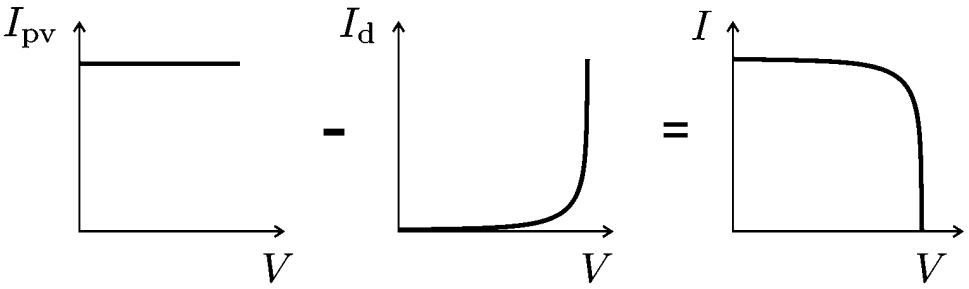
\includegraphics[width=\textwidth]{resources/superp.png}
      \caption{Le courant I est la superposition de $I_{PV}$ et de $I_D$ \cite{Villalva2009}}
  \end{subfigure}
  \caption{Modèle idéal d'une cellule PV}
  \label{fig:idealcell}
\end{figure*}

\section{Les modèles simple diode \texorpdfstring{$R_S\ \text{et}\ R_P$}{Rs et Rp}}
Le modèle idéal précèdent est utile pour éclaircir le concept de la modélisation par circuits d'éléments localisés. Par contre, dans la pratique, et pour plus de précision, il est nécessaire de considérer les pertes ohmique de la cellule dans le matériau semi-conducteur utilisé et dans les contacts des électrodes. La manière la plus directe de modéliser ces phénomènes est de tout simplement ajouter une résistance en série $R_S$ au circuit idéal. Ceci nous laisse avec la relation modifiée \ref{eq:singlers} du modèle dit \textit{"simple diode-$R_S$"} qui a besoin de 4 paramètres pour une description complète: $I_{PV}$, $a$, $I_0$ et $R_S$.\\
L'une des limites de ce modèle provient de son imprécision lorsque la cellule subit des variations non-négligeables de température. L'insertion d'une résistance shunt permet d'améliorer la sensibilité du modèle aux variations de température et en même temps de considérer tout courant de fuite pouvant traverser la jonction \cite{Chin2015b}. On se retrouve cette fois avec les 5 paramètres du modèle dit \textit{"simple diode-$R_P$"} ou tout simplement \textit{"simple diode"}: $I_0$, $I_{PV}$, $a$, $R_s$ et $R_P$. La relation entre ces paramètres est décrite par l'équation \ref{eq:single}. Ce modèle offre un compromis entre la simplicité et la précision et par conséquent est très largement testé et utilisé dans la littérature \cite{Carrero2007}. Le diagramme du circuit de ce modèle est présenté dans la figure \ref{fig:single}.

\begin{equation}
  \label{eq:singlers}
  I = I_{PV} - I_0 \bigg[e^{\big(\frac{q(V + RS)}{akT}\big)} - 1\bigg]
\end{equation}

\begin{equation}
  \label{eq:single}
  I = I_{PV} - I_0 \bigg[e^{\big(\frac{q(V + RS)}{akT}\big)} - 1\bigg] - \frac{V + I R_S}{R_P}
\end{equation}

\begin{figure}
  \begin{center}
    \shorthandoff{:!}
    \resizebox{.5\textwidth}{!}{
    \ctikzset{bipoles/thickness=1}
    \begin{circuitikz}[american currents, line width = 1pt]
    \draw (0, 0) to[I, l=$I_{PV}$] (0, 3) -- (2,3) -- (3,3) to[R=$R_S$, i=$I$] (7,3);
    \draw (7,3) to[open, v^<=$V_{out}$, o-o] (7,0);
    \draw (1.5, 3) to[D, i>^=$I_D$] (1.5, 0);
    \draw (3, 3) to[R=$R_{p}$] (3, 0);
    \draw (0, 0) -- (7, 0);
    \end{circuitikz}}
    \shorthandon{:!}
    \caption{Modèle Simple Diode}
    \label{fig:single}
  \end{center}
\end{figure}



\section{Modèle double diode}

Jusque là on a graduellement amélioré la performance et la précision des modèles de cellules PV en considérant de plus en plus de phénomènes physique qui se produisent dans la cellule (pertes ohmiques, effets des variations de température et courants de fuites). Un phénomène potentiellement influent qui n'est pas considéré par le modèle simple diode est celui des recombinaisons. Comme son nom l'indique, le modèle \textit{"double diode"} (figure \ref{fig:doublediode} n'est que qu'un modèle simple diode auquel on ajoute une autre diode en shunt pour mieux modéliser les effets de recombinaisons surtout aux conditions d'illumination faible \cite{Chin2015b}.\\
Il est évident que l'addition d'une autre diode complique considérablement le modèle et on se retrouve avec deux paramètres supplémentaires ($I_{PV}$, $I_{01}$, $I_{02}$, $a1$, $a2$, $R_S$ et $R_P$). Toutefois, dans les cas où la complexité des calculs associés n'est pas contraignante, la précision de se modèle est supérieure. L'équation \ref{eq:doublediode} décrit la relation entre les 7 paramètres du modèle.

\begin{equation}
  \label{eq:doublediode}
  I = I_{PV} - I_{01} \bigg[e^{\big(\frac{q(V + RS)}{a_1kT}\big)} - 1\bigg] - I_{02} \bigg[e^{\big(\frac{q(V + RS)}{a_2kT}\big)} - 1\bigg] - \frac{V + I R_S}{R_P}
\end{equation}

\begin{figure}[b]
  \begin{center}
    \shorthandoff{:!}
    \resizebox{.5\textwidth}{!}{
    \ctikzset{bipoles/thickness=1}
    \begin{circuitikz}[american currents, line width = 1pt]
      \draw (0, 0) to[I, l=$I_{PV}$] (0, 3) -- (2,3) -- (4.5,3) to[R=$R_S$, i=$I$] (7,3);
      \draw (1.5, 3) to[D, i>^=$I_{D1}$] (1.5, 0);
      \draw (3, 3) to[D, i>^=$I_{D2}$] (3, 0);
      \draw (4.5, 3) to[R=$R_{p}$] (4.5, 0);
      \draw (7,3) to[open, v^<=$V_{out}$, o-o] (7,0);
      \draw (0, 0) -- (7, 0);
    \end{circuitikz}}
    \shorthandon{:!}
    \caption{Le modèle double diode}
    \label{fig:doublediode}
  \end{center}
\end{figure}

\section{Influence des paramètres des modèles}
Chacun des paramètres affecte le comportement du la cellule et la forme de la courbe caractéristique d'une manière différente. Tout d'abord, il faut noter que depuis l'équation \ref{eq:single}, au point court-circuit, on peut négliger le courant de saturation $I_0$ devant le photo-courant $I_{PV}$ qui est supérieur de plusieurs ordres de grandeur. Cette simplification mène au fait que le photo-courant détermine le courant court-circuit de la diode et $I_{PV} \approx I_{CC}$. C'est en fait une simplification que plusieurs méthodes analytiques emploient \cite{Tsai2008, Villalva2009}. En ce qui concerne la résistance série $R_S$, l'augmenter engendre une chute de tension entre la jonction et la sortie de la cellule. On voit dans la figure \ref{fig:rinf} la courbe se rapproche de plus en plus du comportement d'une résistance simple et que des valeurs très grande de $R_S$ entraînent même une diminution légère de $I_{SC}$.

Pour la résistance shunt $R_P$, sa diminution conduit à un détournement d'un partie de plus en plus importante du courant sortant de la jonction, à travers la résistance en parallèle. Le courant total étant constant, le courant de sortie se retrouve de plus en plus réduit. Et comme dans le cas de la résistance série, une cellule avec beaucoup de pertes shunt à un comportement de plus en plus résistif (figure \ref{fig:rinf}.b).

L'équation de Shockley (équation \ref{eq:shockley}) est en fait retrouvée en négligeant toute recombinaison des porteurs de charges dans la zone de déplétion. Dans les diodes et les transistors réels, on constate une différence entre les courbes I-V et le modèle de Shockley \cite{Shockley1949}. Effectivement, le facteur d'idéalité modélise cette déviation du cas idéal. Une diode idéale est marquée par un facteur d'idéalité $a = 1$ alors qu'une diode où les évènements de recombinaison dominent dans la zone de déplétion est marquée par $a = 2$. EXPLAIN WHY Voc DECREASES + SAT CURRENT

\begin{figure*}[h]
  \begin{subfigure}[b]{.48\textwidth}
    \begin{center}
      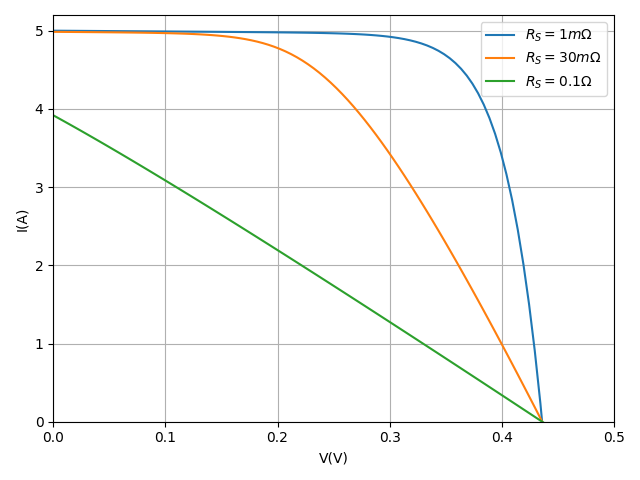
\includegraphics[width=\textwidth]{resources/rsinf.png}
      \caption{Influence de $R_S$}
    \end{center}
  \end{subfigure}
  ~
  \begin{subfigure}[b]{.48\textwidth}
    \begin{center}
      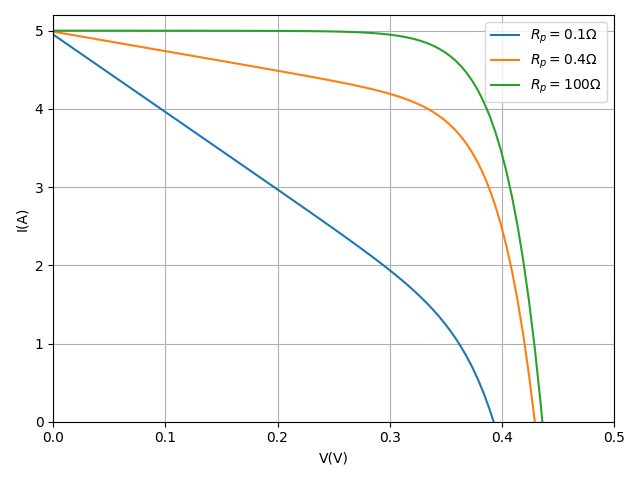
\includegraphics[width=\textwidth]{resources/rpinf.png}
      \caption{Influence de $R_P$}
    \end{center}
  \end{subfigure}
  \caption{Influences de résistances du modèle sur la courbe caractéristique}
  \label{fig:rinf}
\end{figure*}

\begin{figure*}[h]
  \begin{subfigure}[b]{0.48\textwidth}
    \begin{center}
      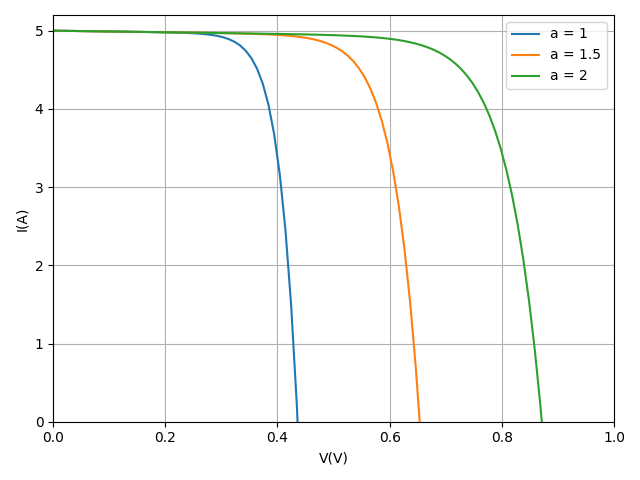
\includegraphics[width=\textwidth]{resources/ainf.png}
      \caption{Influence du facteur d'idéalité}
    \end{center}
  \end{subfigure}
  ~
  \begin{subfigure}[b]{0.48\textwidth}
    \begin{center}
      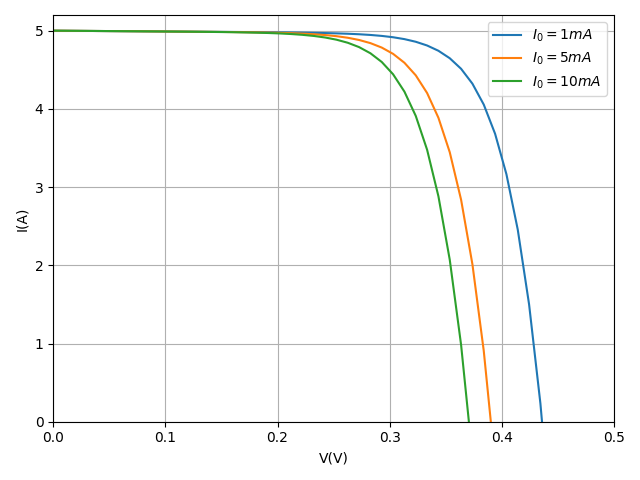
\includegraphics[width=\textwidth]{resources/i0inf.png}
      \caption{Influence du courant de saturation}
    \end{center}
  \end{subfigure}
  \caption{Influence des paramètres de la diode sur la courbe I-V}
  \label{fig:dinf}

\end{figure*}
  
\section{État de l'art d'estimation des paramètres}

Les paramètres (soit les valeurs des éléments localisés des circuits) représentent une description complète du modèle et une bonne estimation de leurs valeurs est essentielle avant leur application. On utilise souvent les données des data-sheets offertes par les fabricants des cellules et modules PV. Ces données couvrent les points clés de la caractéristique I-V (court-circuit, circuit ouvert et puissance maximale). Les méthodes analytiques tendent à utiliser ces informations en plus de quelques expressions comme la pente de la courbe aux points clés pour déterminer les résistances en shunt $R_P$ et en série $R_S$. On trouve souvent aussi des simplifications comme le fait de considérer que seuls les $I_{PV}$ et $I_0$ sont significativement influents sur la caractéristique \cite{Ciulla2014}.
Dans le modèle simple diode contenant les 5 paramètres $I_{PV}$, $I_0$, $a$, $R_S$ et $R_P$, il est très courant de tout simplement négliger $I_0$ devant $I_{PV}$ au point court circuit, et par conséquent considérer que $I_{PV} = I_{CC}$ (La valeur de $I_0$ est ensuite extraite des conditions circuit ouvert) \cite{Villalva2009,Ciulla2014,Tsai2008}. En ce qui concerne $a$, $R_S$ et $R_P$, on a besoin de davantage d'équations. Généralement, les chercheurs utilisent soit les dérivées de la caractéristique aux points clés, soit des expressions analytiques des coefficients de température le liant avec les paramètres.\\
Le problème étant de nature non-linéaire, les techniques d'optimisation avec des capabilités de recherche globales dans l'espace de recherche s'offrent comme alternative. La précision de ces techniques dépends évidemment de la fonction objectif considérée, des conditions initiales et de la nature de l'algorithme lui-même \cite{Easwarakhanthan1986, El-Naggar2012, DaCosta2010}. Les techniques de calcul souple et les algorithmes évolutionnistes ont susciter beaucoup d'intérêt récemment dans la littérature dans le but d'estimer les paramètres des cellules PV. Des techniques de réseaux de neurones artificiels \cite{Balzani2005, Zhang2005a, Karatepe2006}, logique floue \cite{Elhagry1997, Bendib2013, AbdulHadi2004}, algorithme génétique \cite{Jervase2001, Moldovan2009, Ismail2013}, optimisation par essaims particulaires (Particle Swarm Optimization) \cite{Ye2009, Soon2012} et évolution différentielle \cite{DaCosta2010, Ishaque2012, Gong2013} ont été utilisées. Par contre elles ne sont pas utilisées par les simulateurs PV, qui sont contraints par des critères de consistance et de temps de calcul, à cause de leurs nature stochastique. Ceci dit, elles sont très utiles lorsqu'il y a un besoin de précision sur les paramètres pour servir à l'optimisation du processus de fabrication ou pour l'étude de dégradation des cellules \cite{Ikegami2001,Balzani2005}. Dans les chapitres suivants nous allons présenter et analyser une méthode utilisant l'algorithme d'évolution différentielle qui est relativement récente en la comparant avec d'autre algorithmes similaires.

\section{Conclusion}
